\chapter{Specifikacija programske potpore}
		
	\section{Funkcionalni zahtjevi}
			
			
			\noindent \textbf{Dionici:}
			
			\begin{packed_enum}
				
				\item Neregistrirani korisnik
				\item Registrirani korisnik
				\begin{packed_item}
					\item[a)] Sklonište
				\end{packed_item}
				\item Razvojni tim
				
			\end{packed_enum}
			
			\noindent \textbf{Aktori i njihovi funkcionalni zahtjevi:}
			
			
			\begin{packed_enum}
				\item  \underbar{Neregistriran/neprijavljen korisnik (inicijator) može:}
				\begin{packed_enum}
					\item pregledavati aktivne oglase
					\item pretraživati aktivne oglase
					\item registrirati se
					\item prijaviti se u sustav (za postojećeg korisnika)
					\item detaljnjije pregledati oglas i komunikacije
				\end{packed_enum}
			
				\item  \underbar{Registriran/prijavljen korisnik (inicijator) može:}
				\begin{packed_enum}
					\item pregledavati sve oglase
					\item pretraživati sve oglase
					\item detaljnije pregledati oglas i komunikacije
					\item komunikacirati u vezi potrage
					\item postaviti oglas
					\item ukloniti oglas
					\item izmjeniti oglas
				\end{packed_enum}
				
				\item  \underbar{Sklonište (inicijator) može:}
				\begin{packed_enum}
					\item pregledavati sve oglase
					\item pretraživati sve oglase
					\item detaljnijije pregledati oglas i komunikacije
					\item komunicirati u vezi potrage
					\item ukloniti oglas
					\item izmijeniti oglasa
					\item postaviti oglas o ljubimcu u skloništu
				\end{packed_enum}
				
				\item  \underbar{Baza podataka (sudionik) može:}
				\begin{packed_enum}
					\item pohranjivati sve podatke o korisničkim računima
					\item pohranjivati sve podatke o oglasima nestalih ljubimaca
					\item pohranjivati komunikaciju o nestalim ljubimcima
				\end{packed_enum}
				
			\end{packed_enum}
			
			\eject 
			
			
				
			\subsection{Obrasci uporabe}
				
				
				\subsubsection{Opis obrazaca uporabe}
					
					\noindent \underbar{\textbf{UC1 -Registracija}}
					\begin{packed_item}
	
						\item \textbf{Glavni sudionik: } neregistriran korisnik
						\item  \textbf{Cilj:} stvoriti korisnički račun za pristup aplikaciji
						\item  \textbf{Sudionici:} baza podataka
						\item  \textbf{Preduvjet:} -
						\item  \textbf{Opis osnovnog tijeka:}
						
						\item[] \begin{packed_enum}
	
							\item korisnik odabire opciju za registraciju
							\item korisnik unosi potrebne korisničke podatke
							\item korisnik prima obavijest o uspješnoj registraciji
							\item unos podataka u bazu podataka
						\end{packed_enum}
						
						\item  \textbf{Opis mogućih odstupanja:}
						
						\item[] \begin{packed_item}
	
							\item[2.a] odabir već zauzetog korisničkog imena ili emaila, unos korisničkih podataka u nedozvoljenom formatu
							\item[] \begin{packed_enum}
								\item sustav obavještava korisnika o neuspjelom upisu i vraća ga na stranicu za registraciju
								\item korisnik mijenja potrebne podatke te završava unos ili odustaje od registracije
							\end{packed_enum}
							
						\end{packed_item}
					\end{packed_item}
					
					\noindent \underbar{\textbf{UC2 -Prijava}}
					\begin{packed_item}
						
						\item \textbf{Glavni sudionik: } registriran korisnik
						\item  \textbf{Cilj:} prijava u postojeći korisnički račun za pristup aplikaciji
						\item  \textbf{Sudionici:} baza podataka
						\item  \textbf{Preduvjet:} registracija
						\item  \textbf{Opis osnovnog tijeka:}
						
						\item[] \begin{packed_enum}
							
							\item korisnik odabire opciju za prijavu
							\item korisnik unosi korisničko ime i lozinku
							\item potvrda o ispravnosti unesenih podataka
							\item pristup korisničkim funkcijama
						\end{packed_enum}
						
						\item  \textbf{Opis mogućih odstupanja:}
						
						\item[] \begin{packed_item}
							
							\item[3.a] neispravno korisničko ime ili lozinka
							\item[] \begin{packed_enum}
								\item sustav obavještava korisnika o neuspjelom upisu
								\item vraćanje na stranicu za prijavu
							\end{packed_enum}
							
						\end{packed_item}
					\end{packed_item}
					
					\noindent \underbar{\textbf{UC3 -Pregled oglasa}}
					\begin{packed_item}
						
						\item \textbf{Glavni sudionik: } neregistriran korisnik, registriran korisnik
						\item  \textbf{Cilj:} pregledati oglase
						\item  \textbf{Sudionici:} baza podataka
						\item  \textbf{Preduvjet:} -
						\item  \textbf{Opis osnovnog tijeka:}
						
						\item[] \begin{packed_enum}
							
							\item oglasi su prikazani prilikom učitavanja aplikacije
							\item korisnik pregledava oglase
						\end{packed_enum}
						
					\end{packed_item}
					
					\noindent \underbar{\textbf{UC4 -Pretraživanje aktivnih oglasa}}
					\begin{packed_item}
						
						\item \textbf{Glavni sudionik: } neregistriran korisnik, registriran korisnik
						\item  \textbf{Cilj:} pronaći željeni aktivni oglas
						\item  \textbf{Sudionici:} baza podataka
						\item  \textbf{Preduvjet:} -
						\item  \textbf{Opis osnovnog tijeka:}
						
						\item[] \begin{packed_enum}
							
							\item korisnik odabire opcije za pretraživanje
							\item korisnik unosi željene podatke o kategorijama
							\item korisnik odabire opciju "Pretraži"
							\item prikaz pronađenih oglasa
						\end{packed_enum}
						
						\item  \textbf{Opis mogućih odstupanja:}
						
						\item[] \begin{packed_item}
							
							\item[3.a] nijedan oglas ne ispunjava kriterije pretrage
							\item[] \begin{packed_enum}
								\item korisnika se obavještava da nema pronađenih oglasa
							\end{packed_enum}
							
						\end{packed_item}
					\end{packed_item}
					
					\noindent \underbar{\textbf{UC5 -Pretraživanje neaktivnih oglasa}}
					\begin{packed_item}
						
						\item \textbf{Glavni sudionik: } registriran korisnik
						\item  \textbf{Cilj:} pronaći željeni neaktivni oglas
						\item  \textbf{Sudionici:} baza podataka
						\item  \textbf{Preduvjet:} prijava
						\item  \textbf{Opis osnovnog tijeka:}
						
						\item[] \begin{packed_enum}
							
							\item korisnik odabire opcije za pretraživanje
							\item korisnik unosi željene podatke o kategorijama
							\item korisnik odabire opciju "Pretraži"
							\item prikaz pronađenih oglasa
						\end{packed_enum}
						
						\item  \textbf{Opis mogućih odstupanja:}
						
						\item[] \begin{packed_item}
							
							\item[3.a] nijedan oglas ne ispunjava kriterije pretrage
							\item[] \begin{packed_enum}
								\item korisnika se obavještava da nema pronađenih oglasa
							\end{packed_enum}
							
						\end{packed_item}
					\end{packed_item}
					
					\noindent \underbar{\textbf{UC6 - Postavljanje oglasa}}
					\begin{packed_item}
						
						\item \textbf{Glavni sudionik: } registriran korisnik
						\item  \textbf{Cilj:} postaviti oglas o izgubljenom kućnom ljubimcu
						\item  \textbf{Sudionici:} baza podataka
						\item  \textbf{Preduvjet:} prijava
						\item  \textbf{Opis osnovnog tijeka:}
						
						\item[] \begin{packed_enum}
							
							\item korisnik odabire opciju za postavljanje novog oglasa
							\item korisnik korisnik unosi informacije o nestalom ljubimcu
							\item automatsko povlačenje korisničkih podataka
							\item korisnik odabire opciju za objavu
							\item spremanje podataka u bazu podataka
						\end{packed_enum}
						
						\item  \textbf{Opis mogućih odstupanja:}
						
						\item[] \begin{packed_item}
							
							\item[4.a] neispravan unos jedne ili više kategorija podataka o ljubimcu
							\item[] \begin{packed_enum}
								\item korisnika se vraća na ponovni upis oglasa
							\end{packed_enum}
							
						\end{packed_item}
					\end{packed_item}
					
					\noindent \underbar{\textbf{UC7 - Komunikacija oko potrage}}
					\begin{packed_item}
						
						\item \textbf{Glavni sudionik: } registriran korisnik
						\item  \textbf{Cilj:} razmjena informacija o određenom izgubljenom ljubimcu
						\item  \textbf{Sudionici:} baza podataka
						\item  \textbf{Preduvjet:} prijava, postojeći aktivni oglas
						\item  \textbf{Opis osnovnog tijeka:}
						
						\item[] \begin{packed_enum}
							
							\item korisnik odabire opciju za komunikaciju
							\item korisnik korisnik unosi informacije, sliku i lokaciju nestalog ljubimca
							\item korisnik odabire opciju za slanje
							\item nove informacije se prikazuju svim korisnicima
							\item spremanje u bazu podataka
						\end{packed_enum}
						
					\end{packed_item}
					
					\noindent \underbar{\textbf{UC8 - Detaljni pregled oglasa i komunikacije}}
					\begin{packed_item}
						
						\item \textbf{Glavni sudionik: } neregistriran korisnik, registriran korisnik
						\item  \textbf{Cilj:} pregled svih informacija i dosadašnje komunikacije o određenom ljubimcu
						\item  \textbf{Sudionici:} baza podataka
						\item  \textbf{Preduvjet:}
						\item  \textbf{Opis osnovnog tijeka:}
						
						\item[] \begin{packed_enum}
							
							\item korisnik odabire opciju „Prikaži više“
							\item prikaz svih podataka i komunikacije
						\end{packed_enum}
						
					\end{packed_item}
					
					\noindent \underbar{\textbf{UC9 - Uklanjanje vlastitih oglasa}}
					\begin{packed_item}
						
						\item \textbf{Glavni sudionik: } registriran korisnik
						\item  \textbf{Cilj:} ukloniti postojeći oglas s popisa vidljivih oglasa
						\item  \textbf{Sudionici:} baza podataka
						\item  \textbf{Preduvjet:} prijava, pregled vlastitih oglasa, postojeći vlastiti oglas
						\item  \textbf{Opis osnovnog tijeka:}
						
						\item[] \begin{packed_enum}
							
							\item korisnik odabire opciju za uklanjanje oglasa
							\item nestanak oglasa s liste vidljivih oglasa
							\item ažuriranje baze podataka
						\end{packed_enum}
						
					\end{packed_item}
					
					\noindent \underbar{\textbf{UC10 - Izmjena vlastitih oglasa}}
					\begin{packed_item}
						
						\item \textbf{Glavni sudionik: } registriran korisnik
						\item  \textbf{Cilj:} izmijeniti  željene kategorije podataka o ljubimcu i kategoriju vlastitog oglasa
						\item  \textbf{Sudionici:} baza podataka
						\item  \textbf{Preduvjet:} prijava, pregled vlastitih oglasa, postojeći vlastiti oglas
						\item  \textbf{Opis osnovnog tijeka:}
						
						\item[] \begin{packed_enum}
							
							\item korisnik odabire opciju za izmjenu oglasa
							\item korisnik izmjenjuje podatke ili kategoriju oglasa o ljubimcu
							\item korisnik odabire opciju za spremanje promjena
							\item ažuriranje baze podataka
						\end{packed_enum}
						
					\end{packed_item}
					
					\noindent \underbar{\textbf{UC11 - Oglašavanje ljubimaca u skloništu}}
					\begin{packed_item}
						
						\item \textbf{Glavni sudionik: } sklonište
						\item  \textbf{Cilj:} obavijestiti u kojem se skloništu nalazi nestali ljubimac
						\item  \textbf{Sudionici:} baza podataka
						\item  \textbf{Preduvjet:} prijava
						\item  \textbf{Opis osnovnog tijeka:}
						
						\item[] \begin{packed_enum}
							
							\item odabir opcije za postavljanje novog oglasa
							\item unos informacija o nestalom ljubimcu
							\item automatsko povlačenje korisničkih podataka
							\item odabir opcije za objavu
							\item spremanje podataka u bazu podataka
						\end{packed_enum}
						
						\item  \textbf{Opis mogućih odstupanja:}
						
						\item[] \begin{packed_item}
							
							\item[4.a] neispravan unos jedne ili više kategorija podataka o ljubimcu
							\item[] \begin{packed_enum}
								\item  vraćanje na ponovni upis oglasa
							\end{packed_enum}
							
						\end{packed_item}
					\end{packed_item}
					
					\noindent \underbar{\textbf{UC12 - Pregled vlastitih oglasa}}
					\begin{packed_item}
						
						\item \textbf{Glavni sudionik: } registriran korisnik, sklonište
						\item  \textbf{Cilj:} pregled vlastitih oglasa koje je korisnik objavio
						\item  \textbf{Sudionici:} baza podataka
						\item  \textbf{Preduvjet:} prijava, postojeći vlastiti oglas
						\item  \textbf{Opis osnovnog tijeka:}
						
						\item[] \begin{packed_enum}
							
							\item korisnik odabire opciju za prikaz vlastitih oglasa
							\item korisnik pregledava sve svoje oglase
						\end{packed_enum}
						
						\item  \textbf{Opis mogućih odstupanja:}
						
						\item[] \begin{packed_item}
							
							\item[1.a] korisnik do sad nije objavio nijedan oglas
							\item[] \begin{packed_enum}
								\item  korisnika se obavještava da nema izrađenih oglasa
							\end{packed_enum}
							
						\end{packed_item}
						
					\end{packed_item}
					
						\noindent \underbar{\textbf{UC13 - Izmjena tuđih oglasa}}
					\begin{packed_item}
						
						\item \textbf{Glavni sudionik: } sklonište
						\item  \textbf{Cilj:} označiti ljubimca s tuđeg oglasa kao smještenog u sklonište
						\item  \textbf{Sudionici:} baza podataka, registriran korisnik
						\item  \textbf{Preduvjet:} prijava, postojeći aktivni oglas
						\item  \textbf{Opis osnovnog tijeka:}
						
						\item[] \begin{packed_enum}
							
							\item odabir opcije za detaljniji pregled tuđeg oglasa
							\item označavanje ljubimca kao smještenog u sklonište
							\item ažuriranje baze podataka
						\end{packed_enum}
						
					\end{packed_item}
					
					
					
					
					
				\subsubsection{Dijagrami obrazaca uporabe}
					
					\subsection{Dijagram baze podataka}
					
					%unos slike
					\begin{figure}[H]
						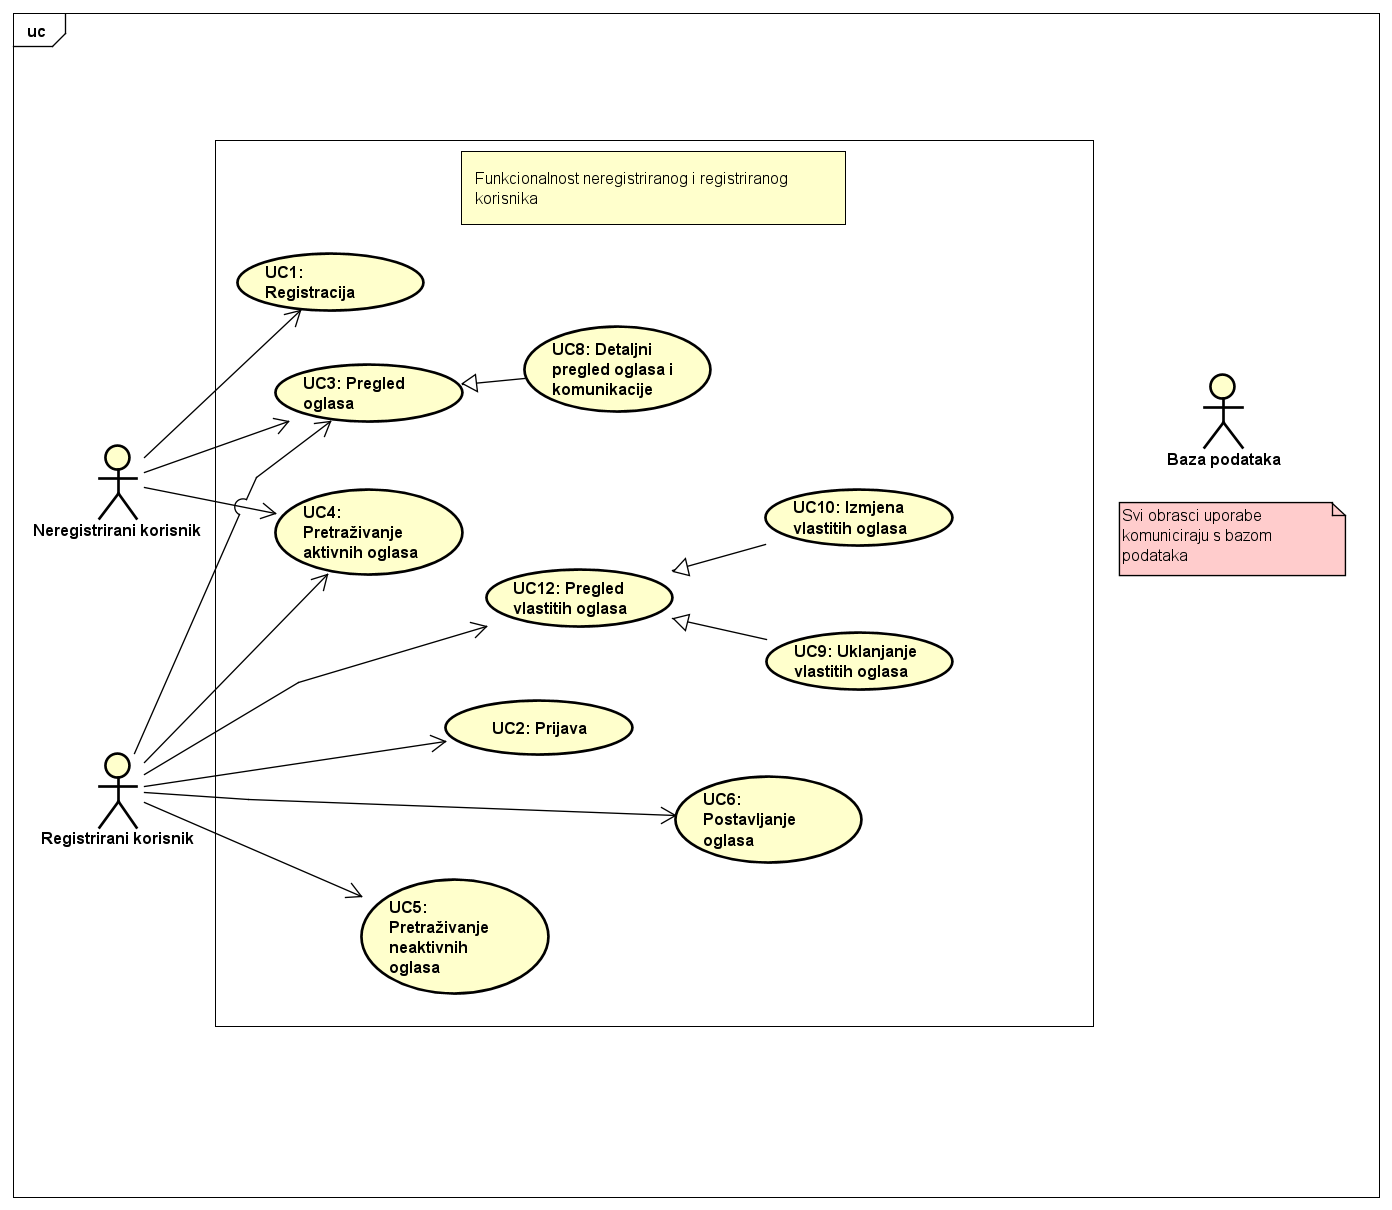
\includegraphics[scale=0.45]{dijagrami/dijagrami obrazaca uporabe/uc dijagram 1} %veličina slike u odnosu na originalnu datoteku i pozicija slike
						\centering
						\caption{Dijagram obrasca uporabe, funkcionalnost neregistriranog i registriranog korisnika}
						\label{fig:ucDijagram1}
					\end{figure}
					
					\begin{figure}[H]
						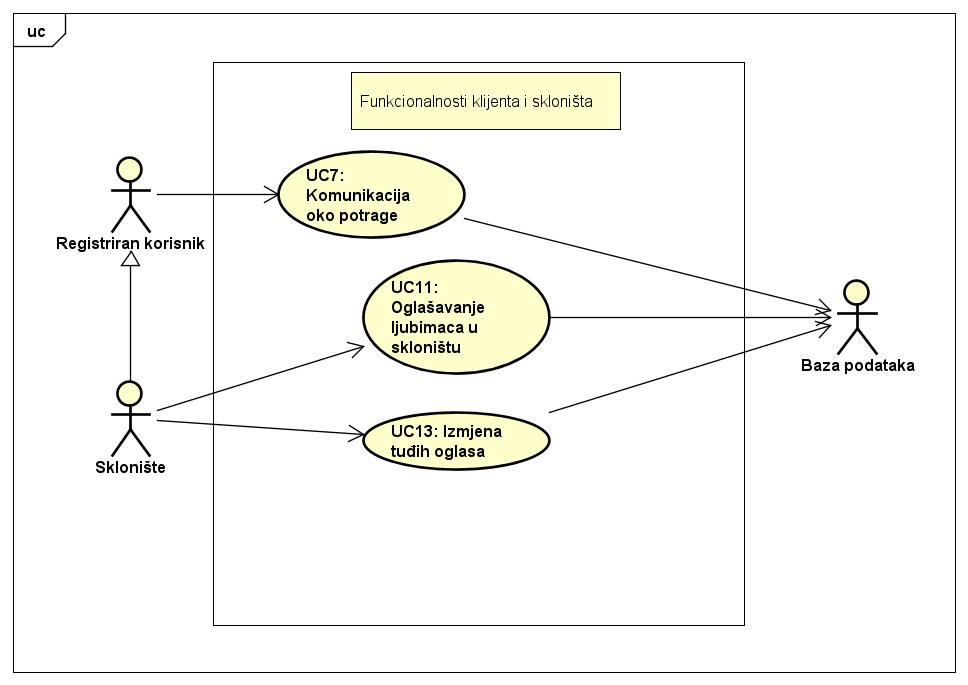
\includegraphics[scale=0.63]{dijagrami/dijagrami obrazaca uporabe/uc dijagram 2} %veličina slike u odnosu na originalnu datoteku i pozicija slike
						\centering
						\caption{Dijagram obrasca uporabe, funkcionalnost skloništa}
						\label{fig:ucDijagram2}
					\end{figure}
					
					\eject
				\eject		
				
			\subsection{Sekvencijski dijagrami}
				
				\textbf{Obrazac uporabe UC4 - Pretraživanje aktivnih oglasa}

				Pokretanjem aplikacije korisnik šalje zahtjev za prikaz aktivnih oglasa. Poslužitelj vraća trenutno aktivne oglase i prikazuje ih. Zatim korisnik odabire opciju za pretraživanje pri čemu mu aplikacija otvara polja za unos filtera. Nakon unosa, korisnik šalje željene filtere poslužitelju koji zatim komunicira s bazom. Ukoliko postoje oglasi koji zadovoljavaju uvjete pretraživanja oni se prikazuju korisniku, a u suprotnom mu se ispisuje odgovarajuća poruka.

					\begin{figure}[H]
						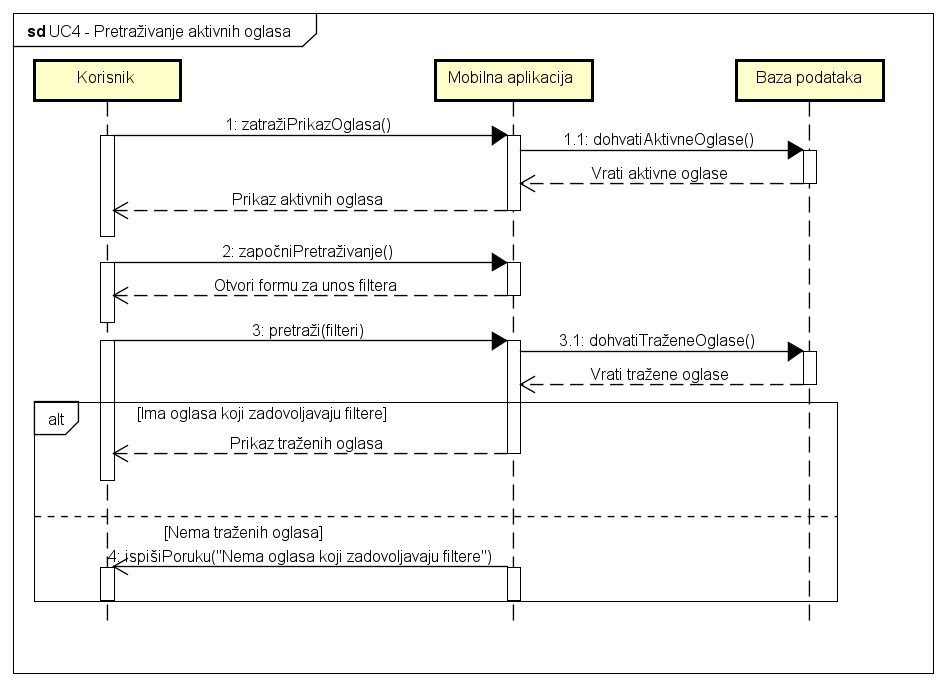
\includegraphics[scale=0.65]{dijagrami/sekvencijskiDijagrami/sd4} %veličina slike u odnosu na originalnu datoteku i pozicija slike
						\centering
						\caption{Sekvencijski dijagram - UC4}
						\label{fig:sDijagram4}
					\end{figure}

				\textbf{Obrazac uporabe UC6 - Postavljanje oglasa}

				Pokretanjem aplikacije korisnik šalje zahtjev za prikaz aktivnih oglasa. Poslužitelj vraća trenutno aktivne oglase i prikazuje ih. Zatim korisnik odabire opciju postavljanja novog oglasa i poslužitelj mu otvara prozor za unos informacija. Korisnik šalje podatke za novi oglas, te poslužitelj provjerava ispravnost unosa. Ako je sve ispravno uneseno, novi oglas se sprema u bazu i prikazuje korisniku. Inače poslužitelj korisnika obavještava o neispravnom unosu podataka.

					\begin{figure}[H]
						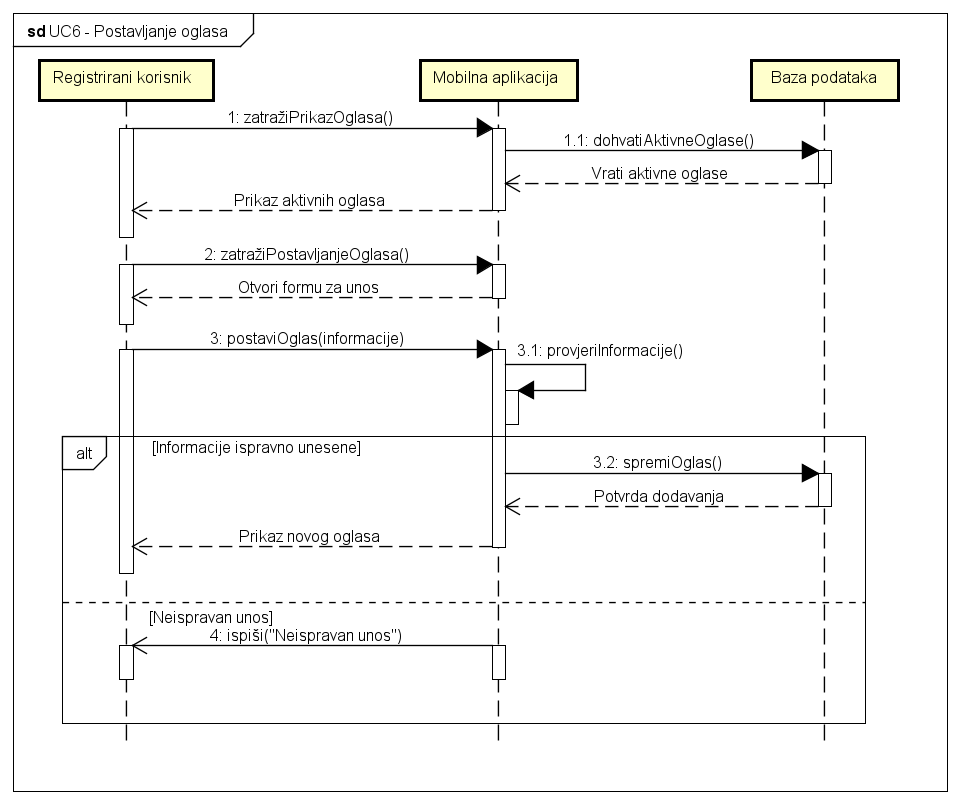
\includegraphics[scale=0.65]{dijagrami/sekvencijskiDijagrami/sd6} %veličina slike u odnosu na originalnu datoteku i pozicija slike
						\centering
						\caption{Sekvencijski dijagram - UC6}
						\label{fig:sDijagram6}
					\end{figure}

				\textbf{Obrazac uporabe UC7 - Komunikacija oko potrage}

				Pokretanjem aplikacije korisnik šalje zahtjev za prikaz aktivnih oglasa. Poslužitelj vraća trenutno aktivne oglase i prikazuje ih. Korisnik odabire oglas, te mu poslužitelj iz baze podataka dohvaća sve informacije o tom oglasu i dosadašnju komunikaciju. Registrirani korisnik može sudjelovati u komunikaciji sve dok ne zatvori odabrani oglas. On unese poruku, šalje je poslužitelju koji je sprema u bazu podataka. Nakon spremanja poruka je vidljiva svim korisnicima.

					\begin{figure}[H]
						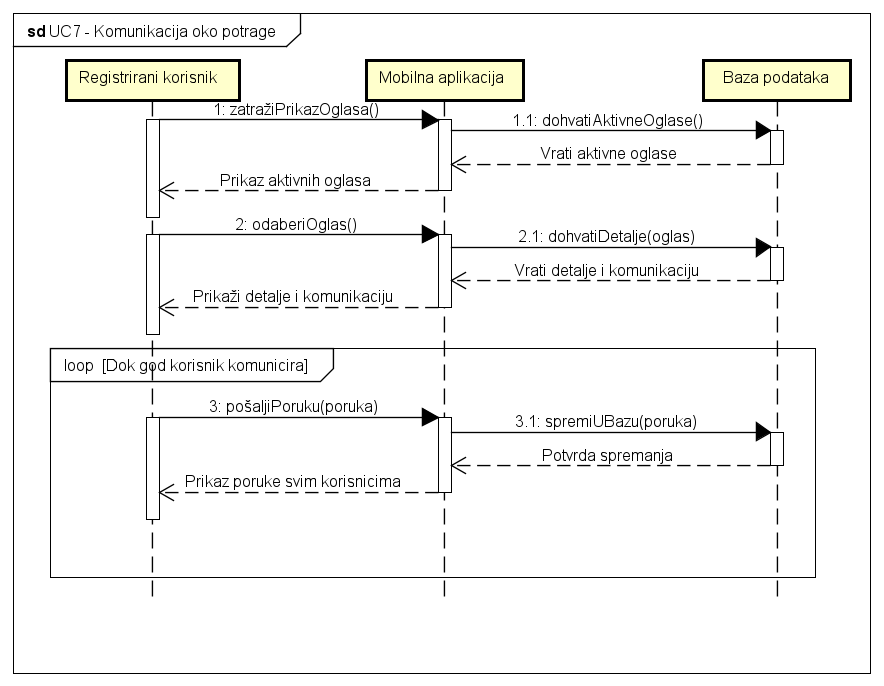
\includegraphics[scale=0.65]{dijagrami/sekvencijskiDijagrami/sd7} %veličina slike u odnosu na originalnu datoteku i pozicija slike
						\centering
						\caption{Sekvencijski dijagram - UC7}
						\label{fig:sDijagram7}
					\end{figure}

				\textbf{Obrazac uporabe UC10 - Izmjena vlastitih oglasa}

				Pokretanjem aplikacije korisnik šalje zahtjev za prikaz aktivnih oglasa. Poslužitelj vraća trenutno aktivne oglase i prikazuje ih. Zatim korisnik traži prikaz njegovih vlastitih oglasa pa ih poslužitelj pokušava dohvatiti iz baze. Ukoliko postoje, prikazuju se u aplikaciji. Sada može odabrati opciju izmjene čime mu poslužitelj otvara prozor za izmjenu oglasa sa svim informacijama o odabranom oglasu iz baze. Registrirani korisnik unosi informacije i šalje ih poslužitelju koji ih zatim provjerava. Ako je sve ispravno uneseno, promjene se spremaju u bazu podataka i izmjenjeni oglas se prikazuje korisniku. Inače, ispisuje mu se poruka o neispravnom unosu. Ako korisnik nije do sada objavio nijedan oglas, ispisuje mu se odgovarajuća poruka.

					\begin{figure}[H]
						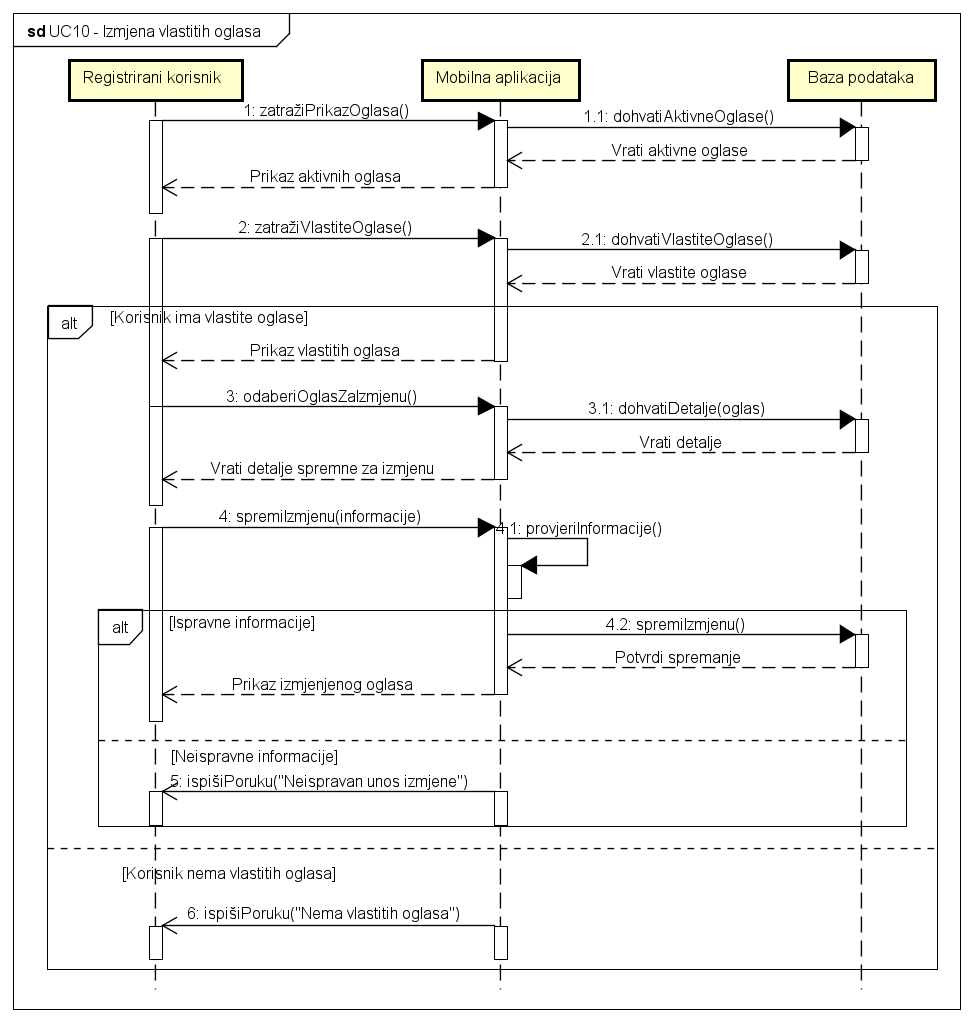
\includegraphics[scale=0.65]{dijagrami/sekvencijskiDijagrami/sd10} %veličina slike u odnosu na originalnu datoteku i pozicija slike
						\centering
						\caption{Sekvencijski dijagram - UC10}
						\label{fig:sDijagram10}
					\end{figure}
				
				\eject
	
		\section{Ostali zahtjevi}
		 
			\begin{packed_item}

				\item  Sustav treba biti implementiran kao mobilna aplikacija koristeći objektno-orijentirane jezike
				\item  Sustav treba podržavati rad više korisnika u stvarnom vremenu
				\item  Administracija podataka obavlja se kroz sučelje baze podataka
				\item  Sustav i korisničko sučelje trebaju podržavati hrvatsku abacedu pri prikazu i unosu tekstualnog sadržaja
				\item  Neispravna upotreba korisničkog sučelja ne smije narušiti funkcionalnost
				\item  Sustav treba biti jednostavan za korištenje svim klijentima
				\item  Veza s bazom podataka treba biti kvalitetno zaštićena, brza i otporna na vanjske greške
				\item  Postojeće funkcionalnosti ne smiju biti narušene pri nadogradnji sustava
				\item  Izvršavanje dijela programa u kojem se pristupa bazi podataka ne smije trajati više od nekoliko sekundi

			\end{packed_item}
			 
			 
			 
	